\section{Introduction}

The blockchain trilemma, also known as the scalability trilemma, refers to the trade-off that exists between decentralization, security, and scalability in blockchain systems. This concept was first proposed by Vitalik Buterin, the co-founder of Ethereum. Ethereum has faced scalability issues due to the limited throughput of the network along with the limitations described by the trilemma. In order to address these issues, various Layer 2 (L2) scalability solutions have been developed for Ethereum. These solutions aim to improve the scalability of the Ethereum network by improving transaction throughput and reducing fees without sacrificing decentralization or security. Polygon zkEVM is a L2 rollup solution that combines data availability and execution verification in the Layer 1 (L1) Ethereum chain to ensure the security and reliability of the L2 state transitions. This document describes the infrastructure designed and implemented by Polygon for this purpose.


\section{Protocol components}
This document aims to describe the protocol used to ensure the finality of the transactions and the correctness of the state transitions in Polygon zkEVM L2 rollup. First we are going to introduce the protocol main components:
\begin{itemize}
	\item \textbf{Trusted Sequencer:} Role responsible for receiving L2 transactions from users, ordering them, generating batches, and submitting them in the form of sequences to L1 contract's storage slots. These batches will be executed and broadcasted to L2 network nodes before in order to achieve fast finality and reduce costs associated with high network usage. Must run a zkEVM node in Sequencer mode and control a specific Ethereum account enforced in L1 contract. 
	\item \textbf{Trusted Aggregator:} Role that takes the L2 batches committed by the Sequencer and uses a special off-chain EVM interpreter that besides being able to compute the L2 State that results from the transaction batches execution, generates a Zero-Knowledge proof of computational integrity (CI). The proof is verified by L1 contracts logic (L1 security inheritance), its successful verification is required to commit the new resulting L2 State root (succinct cryptographic digest of the L2 State) in L1 contract, and it will be an irrefutable proof of that a sequence of batches leads to a specific L2 State. Must run a zkEVM node in Aggregator mode and control a specific Ethereum account enforced in L1 contract.
	\item \textbf{PolygonZkEVM.sol:} L1 contract used by the Sequencer to commit the sequences of transaction batches, acts as historical repository of sequences. Also, allows to the Aggregator to verify publicly the L2 State root transitions by the verification of the transaction batches execution’s proof. Acts as L2 State roots historical repository as well.
\end{itemize}

As shown in Figure 1, batches are generated by the Trusted Sequencer, but to achieve fast finality of L2 transactions and avoid the need to wait for the next L1 block, they are shared with L2 network nodes through a broadcasting channel. Each node will execute the batches to compute locally the resulting L2 State. Then, L2 network nodes will execute again the sequences of batches fetched directly from L1 once they have been committed by the Trusted Sequencer, and therefore they no longer have to trust in it anymore. Eventually, the off-chain execution of the batches will be verified on-chain through the verification of a Zero-Knowledge proof and the resulting L2 State root will be commited. New L2 state roots will also be synchronized by L2 network nodes directly from L1 as final step of the protocol. It is important to note that both data availability and verification of transaction execution rely only on L1 security assumptions and at the final stage of the protocol, the nodes will only rely on data present in L1 to stay synchronized with each L2 State transition.

\begin{center}
	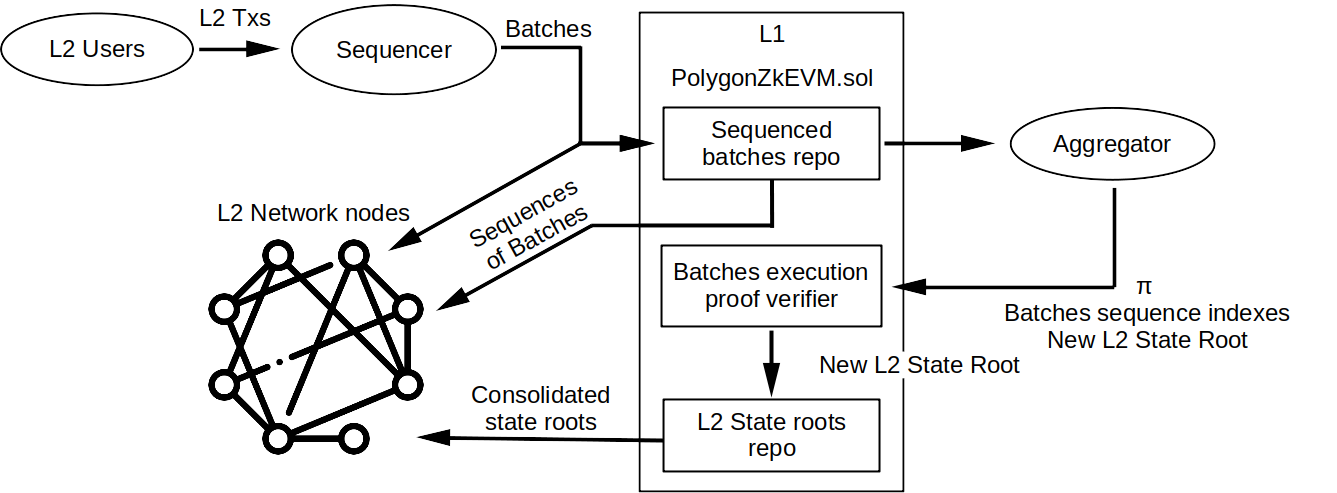
\includegraphics[scale=0.35]{\statemanagementdir/figures/protocol-overview.png}
	
	\captionof{figure}{Polygon zkEVM trustless L2 State management overview.}
\end{center}



\section{L2 State stages}

Since the L2 network nodes update/sync their local state up to a total of 3 times, we have to define 3 possible stages of the L2 State:

\begin{itemize}
	\item \textbf{Trusted state:} State reached when L2 network nodes receive and execute transaction batches broadcasted by the Trusted Sequencer before they are being committed to L1. This stage is called trusted because it is only considered valid based on trust in the Trusted Sequencer.
	

	\item \textbf{Virtual state:} This state is reached when the L2 network nodes process the sequences of batches that have already been submitted to L1 by the Trusted Sequencer. Note that this state is trustless, as it relies on L1 security assumptions. All L2 network nodes can compute their local L2 State by executing the sequences of batches from L1 without relying on the Trusted Sequencer anymore. However, due to different factors that will be explained later, it is possible for the nodes to have divergences between the trusted state and the virtual state. L2 network nodes are prepared to handle these situations and will only consider as valid the state resulting from the execution of the sequences of batches committed in L1.
	\item \textbf{Consolidated state:} State reached when L2 network nodes sync their local L2 State root with that one committed in L1 by the Trusted Aggregator once  Zero-Knowledge proof has verified successfully in L1.
	
\end{itemize}

Figure 2 shows the L2 Stages timeline from a batch perspective and the actions that triggers its inclusion to the next L2 State stage. 

\begin{center}
	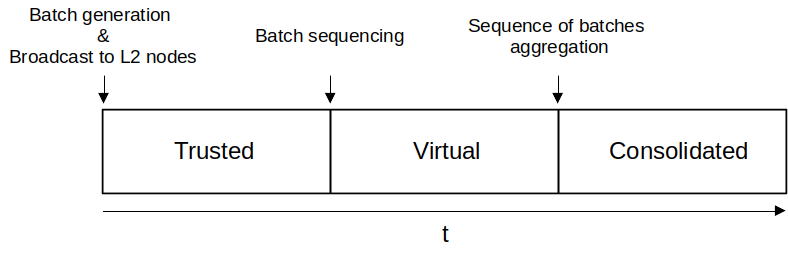
\includegraphics[scale=0.5]{\statemanagementdir/figures/l2-state-stages.png}
	
	\captionof{figure}{L2 State stages timeline.}
\end{center}

\section{zkEVM node execution modes}

zkEVM node is the software package that contains all components needed to run zkEVM network. The node can be run in three different modes:
\begin{itemize}
	\item \textbf{Sequencer:} Holds an instance of L2 State, manages batches broadcasting to other L2 network nodes, and has an API (Application Programming Interface) to handle L2 user's interactions (transaction requests and L2 State queries). Also has a database to temporarily store the transactions that have not yet been ordered and executed (pending transactions pool), and all the components needed to interact with L1 in order to sequence transaction batches, and maintain up-to-date its local L2 State.
	\item \textbf{Aggregator:} Has all the sw components needed to execute transaction batches, compute the resulting L2 State and generate the Zero-Knowledge CI proof. Also, has all the components needed to fetch transaction batches committed in L1 by the Trusted Sequencer and call the functions to verify publicly the L2 State transitions on L1.
	\item \textbf{RPC:} Holds an instance of L2 State that is updated, first with batches broadcasted by the Trusted Sequencer, and then with sequences of batches fetched from the L1 contract. Also has all the components needed to interact with L1 in order to maintain its local L2 State up-to-date and check L2 State roots synchronism.
\end{itemize}

\section{L2 Transactions life flow.}

\subsection{Transaction submission to Trusted Sequencer node.}

As in transactions sent to L1, the transactions are created by the user's wallets and signed with their private key, in fact, one of the properties of an L2 EVM as Polygon zkEVM is that it has exactly the same user experience as Ethereum L1.

The communication between the users and the zkEVM is done through a JSON RPC that is fully compatible with Ethereum RPC. This approach makes that any EVM compatible application, for example a wallet software, is also compatible with zkEVM natively.

Once the transactions are generated and signed, they are sent to the Trusted Sequencer’s node through his JSON RPC interface. The transactions will be stored in the pending transactions pool awaiting to be selected/discarded to be executed by the sequencer.

\subsection{Transactions execution and trusted state.}

Eventually, the Trusted Sequencer will take the transactions from the pool, will order and add them to transaction batches, and will update its local L2 State by the execution of those batches. Once transactions batches are added into the Trusted Sequencer's L2 State instance, they are immediately available to be shared by the broadcast service to other zkEVM nodes to allow them to have access to the trusted state. Note that by relying on the Trusted Sequencer we can archive fast transaction finality (faster than L1), however the resulting L2 State will be in a trusted state until the batch is sequenced in the L1 contract.

Users usually will interact with trusted L2 State, nevertheless, Due to certain protocol characteristics (detailed in the following sections), the verification process for L2 transactions can take a relatively long time, typically around 30 minutes, but in rare cases up to 2 weeks. As a result, users should be aware of the potential risks associated with high-value transactions, particularly those that cannot be reversed, such as transactions that have an impact outside of L2, such as off-ramps, over-the-counter transactions, and alternative bridges.



\subsection{Transactions batching.}

The Trusted Sequencer must batch the transactions using a special format expressed in the L1 PolygonZkEVM.sol contract as the following \textbf{BatchData} struct:

\begin{lstlisting}[language=Solidity]
	struct BatchData {
        bytes transactions;
        bytes32 globalExitRoot;
        uint64 timestamp;
        uint64 minForcedTimestamp;
    }
\end{lstlisting}

\begin{itemize}
	\item \textbf{transactions:} Byte array containing the concatenated batch transactions. Each transaction is encoded following Ethereum pre-EIP-115 or EIP-115 formats using rlp (Recursive-length prefix) standard and is concatenated with the values v,r,s of the signature.
	\begin{itemize}
		\item EIP-155: rlp(nonce, gasprice, gasLimit, to, value, data, chainid, 0, 0,)vrs.
		\item pre-EIP-155: rlp(nonce, gasprice, gasLimit, to, value, data)vrs.
	\end{itemize}

	\item \textbf{globalExitRoot:} Root of the Bridge's Global Exit Merkle Tree that will be synchronized in the L2 State at the beginning of the batch execution, allows bridge claiming transactions to be executed in L2 successfully. The Bridge is used to move assets among L1 and L2, and a claiming transaction is used to unlock the asset in the destination network.
	\item \textbf{timestamp:} Batch timestamp, the max batch timestamp that a Trusted Sequencer can set to a batch is the timestamp of the block where the sequencing L1 transaction is executed. Also, the timestamp of a batch must be higher or equal than the timestamp of the last sequenced batch. These two restrictions constrains the batches to be ordered in time and synchronized  with L1 blocks. 
	\item \textbf{minForcedTimestamp:} This parameter will be different from zero if a batch is a forced batch, a forced batch is used as a censorship countermeasure (detailed in section V).
\end{itemize}


\subsection{Batches sequencing and virtual state.}

To sequence a batch means to successfully add a sequence of batches to L1 PolygonZkEVM.sol contract's mapping \textbf{sequencedBatches}, that is a storage structure that holds the queue of sequences that defines the virtual state.

\begin{lstlisting}[language=Solidity]
	// SequenceBatchNum --> SequencedBatchData
	mapping(uint64 => SequencedBatchData) public sequencedBatches;
\end{lstlisting}

Figure 3 shows the logic structure of a sequence of batches, the quantity of transactions that can be included in a batch is limited by the transaction byte array length to the value of  the contract's \textbf{MAX\_TRANSACTIONS\_BYTE\_LENGTH} (300000) public constant. Likewise, the quantity of batches in a sequence is limited by the contract's \textbf{MAX\_VERIFY\_BATCHES} (1000) public constant.

\begin{center}
	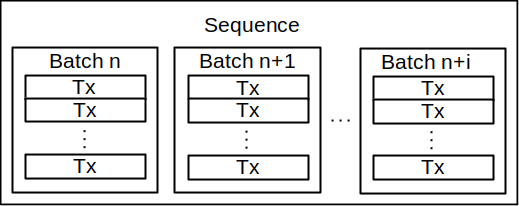
\includegraphics[scale=0.45]{\statemanagementdir/figures/sequence-structure.png}
	\captionof{figure}{Sequence structure.}
\end{center}


To sequence a sequence of batches, the Trusted Sequencer has to call the \textbf{sequenceBatches} contract function, giving as argument an array with the batches to be sequenced.

\begin{lstlisting} [language=Solidity]
	function sequenceBatches(
		BatchData[] memory batches
	) public ifNotEmergencyState onlyTrustedSequencer	
\end{lstlisting}

\textbf{batches} array must contain at least one batch and at most the value of 

\textbf{MAX\_VERIFY\_BATCHES} constant. \textbf{sequenceBatches} can only be called by the Trusted Sequencer's Etherum account. In addition, the contract must not be in emergency state (detailed in section IX). If these conditions are not meet the function call will revert.

 The \textbf{sequenceBatches} function will iterate over every batch of the sequence, checking its validity. A valid batch must meet the following criteria:
\begin{itemize}
	\item Must include a \textbf{globalExitRoot} value that is present in the \textbf{GlobalExitRootMap} of the bridge's L1 PolygonZkEVMGlobalExitRoot.sol. That means that the batch to be sequenced must include a valid globalExitRoot.  

	\item Transactions byte array length must be less than the value of 

\textbf{MAX\_TRANSACTIONS\_BYTE\_LENGTH} constant.
	
	\item The timestamp of the batch must be greater than or equal to that of the last batch sequenced and less than or equal to the timestamp of the block where the sequencing L1 transaction is executed. Note that the batches are ordered by timestamp and that they can never exceed the timestamp of the L1 block in which the sequencing transaction is executed, so L1 block timestamps will act as clock source for L2 batches to achieve time synchronization between both networks.
\end{itemize}

If a batch is not valid the transaction will revert discarding the entire sequence. Otherwise, If the batch is valid the sequencing process will continue.

\textbf{lastBatchSequenced} is a storage variable that will be incremented for each batch sequenced, acts as a batch counter and gives a specific index number to each batch that will be used as a position value in the batch chain.

To ensure the cryptographic integrity of the batch chain, a mechanism will be used to link the batches to their previous one. An accumulated hash will be cumputed for each sequenced batch. It is called accumulated because binds the batch to the accumulated hash of the previous batch sequenced. 

For a specific batch the accumulated hash is computed as follows:

\begin{lstlisting}[language=Solidity]
	keccak256(
		abi.encodePacked(
			currentAccInputHash,
			currentTransactionsHash,
			currentBatch.globalExitRoot,
			currentBatch.timestamp,
			msg.sender))
\end{lstlisting}

\begin{itemize}
	\item \textbf{currentAccInputHash (bytes32):} Accumulated hash of the previous batch sequenced.
	\item \textbf{currentTransactionsHash (bytes32):} Hash digest of the current batch transactions bytes array, keccak256(currentBatch.transactions).
	\item \textbf{currentBatch.globalExitRoot (bytes32):} Bridge's Global Exit Merkle Tree root resulting from the current batch execution.
	\item \textbf{currentBatch.timestamp (uint64):} Current batch timestamp. 
	\item \textbf{msg.sender (address)} EOA that is executing the sequencing transaction in L1.
\end{itemize}

As can be seen in Figure 4, each accumulated hash will ensure the integrity of the batch data (transactions, timestamp, globalExitRoot) and that of all its predecessors, as well as the order in which they have been sequenced. Note that any alteration in the batch chain is not possible since the modification of a single bit would lead to a different last accumulated hash.

\begin{center}
	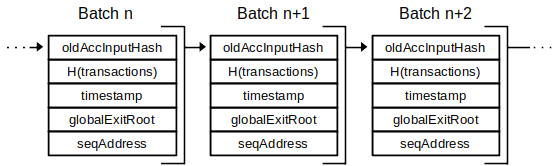
\includegraphics[scale=0.60]{\statemanagementdir/figures/hashchain.png}
	\captionof{figure}{Batch chain structure.}
\end{center}

Once the validity of all batches in the sequence is verified and the accumulated hash of each one has been computed, the batch sequence will be added to \textbf{sequencedBatches} mapping using the following \textbf{SequencedBatchData} struct:

\begin{lstlisting} [language=Solidity]
		struct SequencedBatchData {
			bytes32 accInputHash;
			uint64 sequencedTimestamp;
			uint64 previousLastBatchSequenced;
		}
\end{lstlisting}

\begin{itemize}
	\item \textbf{accInputHash:} Unique batch’s cryptographic representative of the last batch in the sequence.
	\item \textbf{sequencedTimestamp:} Timestamp of the block where the sequencing L1 transaction is executed.
	\item \textbf{previosLastBatchSequenced:} Index of the last sequenced batch before the first batch of the current sequence, i.e. the last batch of the previous sequence.
\end{itemize}

The index number of the last batch in the sequence will be used as key and the \textbf{SequencedBatchData} struct will be used as value when the sequence will be entered in \textbf{sequencedBatches} mapping. Since storage operations in L1 are very expensive in terms of gas consumption, it is important to minimize its use as much as possible. To do this, storage slots (mapping entries) are used exclusively to store a commitment of the sequence. Each entry in the mapping will commit two batch indices (last batch of the previous sequence as value of  \textbf{SequencedBatchData} struct, and last batch of the current sequence as mapping key) along with the accumulated hash of the last batch in the current sequence and a timestamp.

Note that only accumulated hash of last batch in the sequence is stored, all the others are only computed on the fly in order to obtain last one. Indeed, as it si explained above, that hash digest will be a commitment of the entire batch chain. Also, batch indices commit useful information such as the number of batches in the sequence and their position in the batch chain. Timestamp binds the sequence to a specific moment in time.



The data availability of the L2 transactions is guaranteed because the data of each batch can be recovered from the sequencing transaction's calldata, which are not part of the storage of the contract but are part of the L1 State.

The last requirement to complete the execution of the sequencing transaction is that the sequencer pay the sequencing fee stipulated by the incentive mechanism (detailed in section V).

Finally a \textbf{SequenceBatches} event will be emitted.

\begin{lstlisting} [language=Solidity]
	event SequenceBatches(uint64 indexed numBatch)
\end{lstlisting}


 Once the batches are successfully sequenced in L1, all zkEVM nodes can sync their local L2 State state by fetching the sequences of batches directly from L1 PolygonZkEVM.sol contract without the need of trust in the Trusted Sequencer anymore, hence the L2 virtual State is reached.


\subsection{Batches aggregation and consolidated state.}

To avoid future misunderstandings, it is necessary to differentiate between the terms "consolidation", "verification" and "aggregation". While consolidation refers to state transitions or resulting L2 State roots, verification and aggregation refers to the sequences of batches. Moreover, the consolidation of a specific state transition implies, first the successful verification, and then, the successful aggregation of the specific sequence of batches that represents that specific state transition.

To achieve the L2 State final stage (consolidated) the Trusted Aggregator should eventually aggregate the sequences of batches previously committed by the Trusted Sequencer. 

To aggregate a sequence means to successfully add the resulting L2 State root to L1 PolygonZkEVM.sol contract's \textbf{batchNumToStateRoot} mapping, that is a storage structure that holds all the consolidated L2 State roots keyed by last batch index of every aggregated sequence of batches. 

\begin{lstlisting} [language=Solidity]
	// BatchNum --> state root
	mapping(uint64 => bytes32) public batchNumToStateRoot;
\end{lstlisting}

The verification of a sequence of batches implies the successful verification of the Zero-Knowledge CI proof of the sequence of batches execution. The underlying Zero-Knowledge verification schema is a Succinct Non-interactive Arguments of Knowledge (SNARK), and one of its key properties is the succinctness of the proof and its fast verification. Therefore, given an exhaustive computation, its integrity can be verified using a fraction of the computational resources required by the original computation. So that, with the use of a SNARK schema we can give on-chain security to exhaustive off-chain computations in a gas efficient way.

As can be seen in Figure 5, the off-chain execution of a sequence of batches will suppose an L2 state transition and consequently, a change to a new L2 state root. A computation integrity (CI) proof of that execution will be generated by the Aggregator, and its on-chain verification (L1) will ensure the validity of that resulting L2 state root.

\begin{center}
	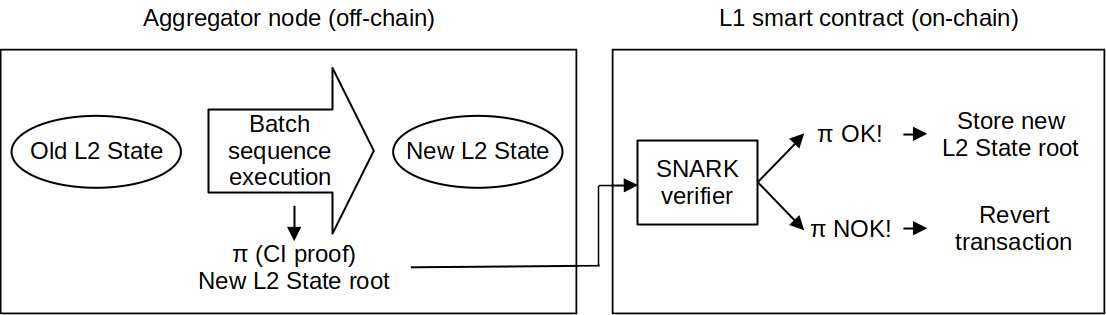
\includegraphics[scale=0.35]{\statemanagementdir/figures/off-chain-execution-on-chain-security.png}
	\captionof{figure}{off-chain L2 state transition with on-chain security inheritance.}
\end{center}



In order to aggregate a sequence of batches, the Trusted Aggregator must call the \textbf{trustedVerifyBatches} contract's function:

\begin{lstlisting} [language=Solidity]
	function trustedVerifyBatches(
		uint64 pendingStateNum,
		uint64 initNumBatch,
		uint64 finalNewBatch,
		bytes32 newLocalExitRoot,
		bytes32 newStateRoot,
		uint256[2] calldata proofA,
		uint256[2][2] calldata proofB,
		uint256[2] calldata proofC
	) public onlyTrustedAggregator 
\end{lstlisting}

\begin{itemize}
	\item \textbf{pendingStateNum:} Number of state transitions pending to be consolidated, 0 as long as the Trusted Aggregator is operating normally. Pending state is a security mechanism used when L2 state is consolidated by an independent Aggregator (detailed in section VII).
	\item \textbf{initNumBatch:} The index of the last batch in the last aggregated sequence.
	\item \textbf{finalNewBatch:} The index of the last batch in the sequence being aggreated.
	\item \textbf{newLocalExitRoot:} The root of the Bridge's L2 Exit Merkle Tree at the end of sequence execution that will be used to compute new Global Exit Root when the sequence will be aggregated, allows bridge claiming transactions to be executed in L1 successfully.
	\item \textbf{newStateRoot:} The L2 StateRoot resulting from the execution of the sequence of batches over an older L2 State.
	\item \textbf{proof (A, B and C):} Zero-Knowledge CI proof of the sequence of batches execution.
\end{itemize}
\textbf{trustedVerifyBatches} can only be called by the Trusted Aggregator account.
Initially \textbf{trustedVerifyBatches} function will call \textbf{\_verifyAndRewardBatches} internal function. \textbf{\_verifyAndRewardBatches} takes the same arguments as \textbf{trustedVerifyBatches} and implements the logic to verify the Zero-Knowledge CI proof of a given sequence of batches execution and, in case of successfully verification, pay the reward stipulated by the incentive mechanism to the aggregator (detailed in section V).

For a sequence of batches to be successfully verified the following conditions must be met:

\begin{itemize}
	\item \textbf{initNumBatch} argument must be the index of an already aggregated batch, that is, must have an L2 State root in \textbf{batchNumToStateRoot} mapping.
	\item \textbf{initNumBatch} argument must be less or equal than last verified batch index.
	\item \textbf{finalNewBatch} argument must be higher than last verified batch index.
	\item \textbf{initNumBatch} and \textbf{finalNewBatch} arguments have to be sequenced batches, that is to be in \textbf{sequencedBatches} mapping.
	\item Zero-Knowledge CI proof must be successfully verified.
\end{itemize}


The Executor and the Prover are services of the Aggregator node that execute batches and generate Zero-Knowledge proofs. Their architecture is beyond the scope of this article, so for now we will treat them as an Ethereum Virtual Machine (EVM) "black box" interpreter that executes a sequence of transaction batches on the current L2 state, calculates the resulting L2 state root, and generates a Zero-Knowledge CI proof for the execution.

The proving/verification system is designed in such a way that, if the proof verification succeeds, is cryptographically proven that the execution of the given sequence of batches over a Specific L2 State leads to an L2 State represented by the \textbf{newStateRoot} argument.

%Looking the arguments of \textbf{verifyBatches} function maybe we can think about the possibility of a fake proof generation because the batch numbers do not represent unequivocally a specific batch in the sequence. Nevertheless, in an early phase of the protocol an unique batch’s cryptographic representative has computed for every sequenced batch (This operation was also done L1, inheriting its security), and these unique identifiers are the ones used in the computation and verification of the proof.

The following code is the part of the PolygonZkEVM.sol contract where the the Zero-Knowledge proof is verified:

\begin{lstlisting}[language=Solidity]
	// Get snark bytes
	bytes memory snarkHashBytes = getInputSnarkBytes(
		initNumBatch,
		finalNewBatch,
		newLocalExitRoot,
		oldStateRoot,
		newStateRoot
	);
	
	// Calulate the snark input
	uint256 inputSnark = uint256(sha256(snarkHashBytes)) % _RFIELD;
	
	// Verify proof
	require(
		rollupVerifier.verifyProof(proofA, proofB, proofC, [inputSnark]),
		"PolygonZkEVM::_verifyBatches: Invalid proof"
	);

\end{lstlisting}

\textbf{rollupVerifier} is an external contract that has a function \textbf{verifyProof} that takes a proof (proofA, proofB, proofC) and a value \textbf{inputSnark} and returns a boolean value that will be true if the proof is valid and false if it isn't. 

The successful verification of the proof just confirms the integrity of the computation, but not that the correct inputs were used and that they resulted in the correct output values. Public arguments are used to publicly disclose key points of the computation being proved, in order to prove that it was performed using the correct inputs and reveal the outputs. 

This way, during the proof verification, the L1 smart contract will set the public arguments to ensure that the state transition being proved corresponds to the execution of the batches committed by the Trusted Sequencer.

\textbf{inputSnark} is an 256 bits unique cryptographic representative of a specific L2 State transition, which is used as public argument. Is computed as sha256 mod \% \_RFIELD  hash of a bytes string called \textbf{snarkHashBytes} (modulo operator is needed due math primitives used in SNARKs). \textbf{snarkHashBytes} array is computed by a smart contract’s function called \textbf{getInputSnarkBytes} and it is an ABI encoded packed string of the following values:
\begin{itemize}
	\item \textbf{msg.sender:} Address of Trusted Aggregator.
	\item \textbf{oldStateRoot:} L2 State Root that represents the L2 State before the state transition that wants to be proven.
	\item \textbf{oldAccInputHash:} Accumulated hash of the last batch aggregated.
	\item \textbf{initNumBatch:} Index of the last batch aggregated.
	\item \textbf{chainID:} Unique chain identifier.
	\item \textbf{newStateRoot:} L2 State Root that represents the L2 State after the state transition that is being proved.
	\item \textbf{newAccInputHash:} Accumulated hash of the last batch in the sequence that is being aggregated.
	\item \textbf{newLocalExitRoot:} Root of the Bridge's L2 Exit Merkle Tree at the end of sequence execution.
	\item \textbf{finalNewBatch:} Number of the final batch in the execution range.
\end{itemize}

\textbf{InputSnark} will represent all the L2 transactions of a specific L2 State transition, executed in a specific order, in a specific L2 (chain id), and proved by a specific Trusted Aggregator (msg.sender). The \textbf{trustedVerifyBatches} function not only verifies the validity of the Zero-Knowledge proof, but it also checks that the value of \textbf{InputSnark} corresponds to an L2 State transition that is pending to be aggregated.

If the internal call to \textbf{\_verifyAndRewardBatches} returns true will mean that the sequence of batches is verified successfully, and then the \textbf{newStateRoot} argument will be added to the \textbf{batchNumToStateRoot} mapping. The index of the last batch in the sequence will be used as the key for the entry.

Finally a \textbf{TrustedVerifyBatches} event will be emitted.

%and the new bridge's Global Exit Root will be computed by L1 PolygonZkEVMGlobalExitRoot.sol contract using \textbf{newLocalExitRoot} argument. Otherwise, the aggregation transaction will revert. Note that this root update is the synchronization source of the bridge from L2 to L1. 

\begin{lstlisting} [language=Solidity]
	event TrustedVerifyBatches(
		uint64 indexed numBatch,
		bytes32 stateRoot,
		address indexed aggregator
	);
\end{lstlisting}

Once the batches are successfully aggregated in L1, all zkEVM nodes can check the validity of  their local L2 State by fetching and checking consolidated roots directly form L1 PolygonZkEVM.sol contract, hence the L2 consolidated State is reached.
 
 
\section{Incentives mechanism}

In order to keep the system sustainable, the actors must be incentivized to perform their role correctly and give finality to the protocol.

\subsection{L2 transaction fees and sequencing fees} 
Bridged Ether, originary from L1, is the native currency used in L2, that is, the currency used to pay L2 transaction fees. It can be bridged from L1 to L2 and viceversa at a 1:1 exchange ratio. Since L2 accounts, by default, do not have ether to pay transaction fees, when claiming bridged assets from L1, L2 claiming transactions that call bridge claiming functions are funded by the protocol and will not require the payment of gas fees.

The sequencer will earn the transaction fees paid by users in L2, so it will be paid directly in bridged ether. The amount of fees paid will depend on the gas price, which is set by users based on how much they are willing to pay for the execution of their transactions.


To incentivize the Aggregator, for every batch sequenced , the Sequencer must lock in L1 PolygonZkEVM.sol contract a quantity of MATIC tokens proportional to the number of batches in the sequence. \textbf{batchFee} storage variable contais the quantity of MATIC tokens that must be locked per batch sequenced.

Figure 6 shows the incomes and the outcomes for each actor in the protocol.


\begin{center}
	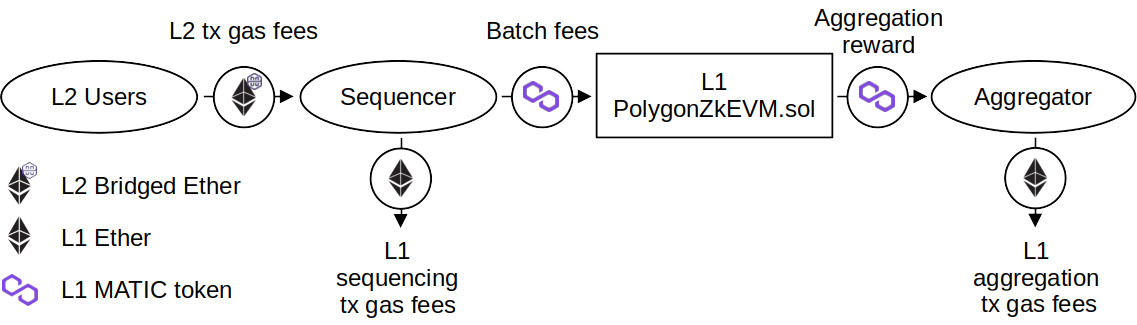
\includegraphics[scale=0.35]{\statemanagementdir/figures/incentives.png}
	\captionof{figure}{Incomes and the outcomes for each actor in the protocol.}
\end{center}

Note that the Sequencer will prioritize transactions with higher gas prices in order to maximize its income. Additionally, there is a threshold below which it would not be profitable for the Sequencer to execute transactions, as the fees earned from L2 users would be less than the equivalent in ether of the amount of MATIC paid as sequencing fees plus L1 sequencing transaction fee. To incentivize the Sequencer, users should set their transaction fees to target a level above this threshold, otherwise the Sequencer will not be incentivized to process their transactions. The following expression represents the net ether value earned by the Sequencer for sequencing a sequence of batches:

$$"Sequencer\:net\:ether\:income" = totalL2TxGasFee - (L1SeqTxGasFees + \frac{batchFee * nBatches}{MATIC/ETH})$$

where:
\begin{itemize}
	\item \textbf{totalL2TxGasFees:} Total sum of fees gathered from all L2 transactions included in the sequence of batches.
	\item \textbf{L1SeqTxGasFee:} Sequencing transaction gas fee paid in L1.
	\item \textbf{batchFee:} PolygonZkEVM.sol \textbf{batchFee} storage variable.
	\item \textbf{nBatches:} Number of batches in the sequence.
	\item \textbf{MATIC/ETH:} Price of MATIC token expressed in ether.
\end{itemize}



\subsection{Aggregation reward}

Every time an Aggregator aggregates a sequence, the quantity of MATIC tokens earned will depend on the total contract MATIC balance and the number of batches being aggregated. The quantity of MATIC earned per batch aggregated is calculated by the L1 PolygonZkEVM.sol contract before the aggregation of a sequence using the following expression:

$$ batchReward = \frac{"contract\:MATIC\:balance"}{"Quantity\:of\:batches\:not\:aggregated\:yet"}$$

Therefore, the following expression represents the total amount of ether value that the Aggregator will earn for the aggregation of a sequence of batches.

$$"Aggregator\:net\:ether\:income" = \frac{batchReward * nBatches}{MATIC/ETH} - L1AggTxGasFee$$

where:
\begin{itemize}
	\item \textbf{L1AggTxGasFee:} Aggregation transaction gas fee paid in L1.
	\item \textbf{batchReward:} quantity of MATIC earned per batch aggregated.
	\item \textbf{nBatches:} Number of batches in the sequence.
	\item \textbf{MATIC/ETH:} Price of MATIC token expressed in ether.
\end{itemize}


\subsection{\textbf{batchFee} variable re-adjustments}

 \textbf{batchFee} will be automatically adjusted every time a sequence is aggregated by an independent Aggregator. This situation occurs when the Trusted Aggregator is not functioning properly (detailed in Section VII), and the \textbf{batchFee} variable will be modified to incentivize aggregation.


\textbf{\_updateBatchFee} internal function is used to adjust \textbf{batchFee} storage variable.

\begin{lstlisting}
	function _updateBatchFee(uint64 newLastVerifiedBatch) internal 
\end{lstlisting}

Two storage variables defined by the Admin (detailed in section IX) are used to tune the fee adjustment function:
\begin{itemize}
	\item \textbf{veryBatchTimeTarget:} Time target of the verification of a batch, the \textbf{batchFee} variable will be updated to achieve this target.
	\item \textbf{multiplierBatchFee:} Batch fee multiplier with 3 decimals that goes from 1000 - 1024.
\end{itemize}

\textbf{\_updateBatchFee} first will evaluate how many of the batches being aggregated are late, that is they are not aggregated yet and \textbf{veryBatchTimeTarget} time has passed. \textbf{diffBatches} variable represents the difference between late batches and the ones below the target nevertheless its value is limited by \textbf{MAX\_BATCH\_MULTIPLIER} constant (12).

If in the sequence being aggregated there are more late batches than other ones below the target, the following formula will be applied to \textbf{batchFee} storage variable:

$$"new\: batch\: fee" = "old\: batch\: fee"\frac{multiplierBatchFee^{diffBatches}}{10^{3\,diffBatches}}$$

Figure 7 shows \textbf{batchFee} variable variation in \% depending on the \textbf{diffBatches} value for different values of \textbf{multiplierBatchFee} when late batches dominate the sequence. Note that the objective is to increase the aggregation reward to incentivize aggregation.

\begin{center}
	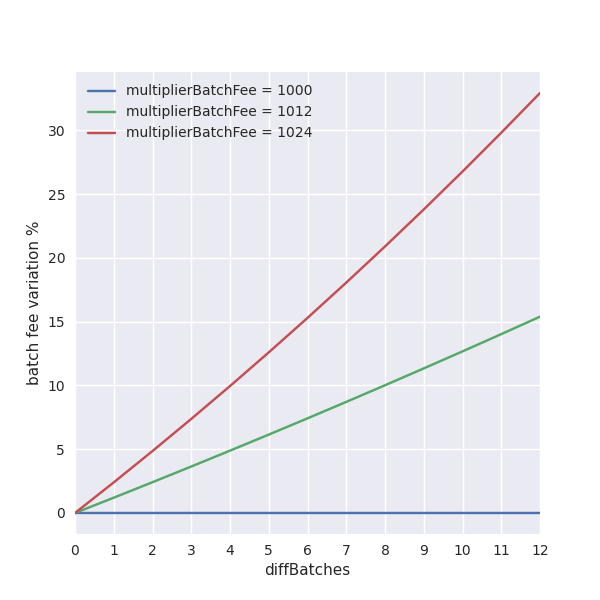
\includegraphics[scale=0.45]{\statemanagementdir/figures/batch-fees-plot-mult.png}
	
	\captionof{figure}{\% of batch fee variation when late batches 
		dominate the sequence.}
\end{center}


In the other case, if there are more batches below the target than late ones , the following formula will be applied to \textbf{batchFee} storage variable:

$$"new\: batch\: fee" = "old\: batch\: fee"\frac{10^{3\,diffBatches}}{multiplierBatchFee^{diffBatches}}$$

Figure 8 shows \textbf{batchFee} variable variation in \% depending on the \textbf{diffBatches} value for different values of \textbf{multiplierBatchFee} when batches below the time target 
dominate the sequence. Note that the objective is to decrease the aggregation reward.

\begin{center}
	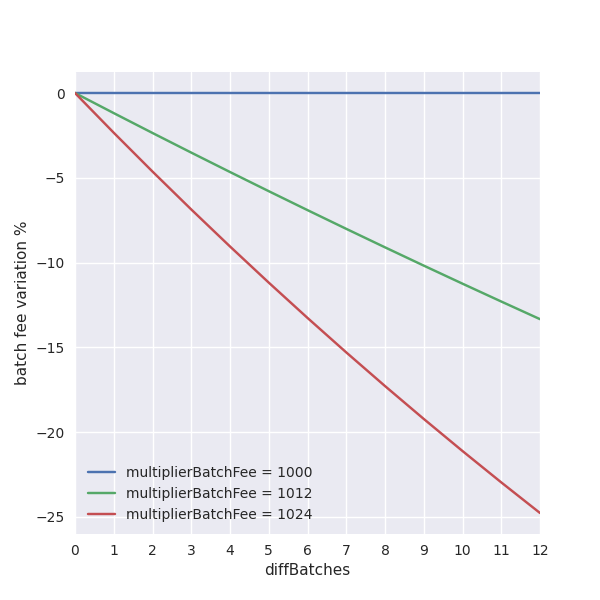
\includegraphics[scale=0.45]{\statemanagementdir/figures/batch-fees-plot-div.png}
	
	\captionof{figure}{\% of batch fee variation when batches below the time target 
		dominate the sequence.}
\end{center}

To sum up with the adjustment of \textbf{veryBatchTimeTarget} and \textbf{multiplierBatchFee} the Admin can tune the reactivity of the \textbf{batchFee} variable re-adjustments and incentivize the protocol's players to target an average \textbf{veryBatchTimeTarget}.

Values set during initialization of the contract:
\begin{itemize}
	\item \textbf{batchFee} = $10^{18}$ (1 MATIC).
	\item \textbf{veryBatchTimeTarget} = 30 minutes.
	\item \textbf{multiplierBatchFee} = 1002.
\end{itemize}



\section{Resistance to Trusted Sequencer censorship or malfunction}

In the scheme described above, the users need to rely in a Trusted Sequencer for their transactions to be executed in the L2. If a user is unable to execute their transactions through the Trusted Sequencer, they can include them in a forced batch. A forced batch is a batch of L2 transactions that users can commit to L1 as a way of publicly declaring their intention to execute those transactions.

\begin{center}
	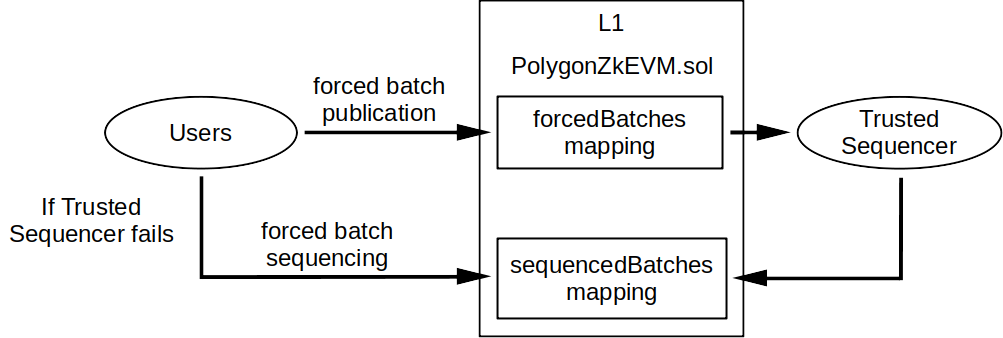
\includegraphics[scale=0.33]{\statemanagementdir/figures/forced-batches.png}
	
	\captionof{figure}{Forced batch sequencing flow.}
\end{center}

As can be seen in Figure 9, PolygonZkEVM.sol contract has a \textbf{forcedBatches} mapping in which the users can submit transaction batches to be forced. \textbf{forcedBatches} mapping acts as immutable notice board in which forced batches will be timestamped and published awaiting to be included in a sequence. In order to maintain its status as a trusted entity, the Trusted Sequencer will include these forced batches in future sequences. Otherwise, users will be able to prove that they are being censored and the Trusted Sequencer will lose its trusted status.   

\begin{lstlisting}[language=Solidity]
	// ForceBatchNum --> hashedForcedBatchData
	mapping(uint64 => bytes32) public forcedBatches;
\end{lstlisting}

Although the Trusted Sequencer is incentivized to sequence the forced batches published in the \textbf{forcedBatches} mapping, this does not guarantee the finality of the execution of the transactions in those batches. To ensure finality in the case of Trusted Sequencer malfunction, the L1 PolygonZkEVM.sol contract has an alternative batch sequencing function called \textbf{sequenceForceBatches}. This function allows anyone to sequence forced batches that have been published in the \textbf{forcedBatches} mapping for a time period specified by the public constant \textbf{FORCE\_BATCH\_TIMEOUT} (5 days) and they have not been sequenced yet.

Any user can publish a batch to be forced by directly calling \textbf{froceBatch} function:

\begin{lstlisting}[language=Solidity]
	function forceBatch(
	bytes memory transactions,
	uint256 maticAmount
	) public ifNotEmergencyState isForceBatchAllowed 
\end{lstlisting}

\begin{itemize}
	\item \textbf{transactions:} Byte array containing the concatenated batch transactions (same as the normal batch transactions format).
	\item \textbf{maticAmount:} Max amount of MATIC tokens that the user is willing to pay as a forced batch publication fee. The fee for publishing a forced batch is the same as the fee for sequencing and is set in the \textbf{batchFee} storage variable. Since the fee is paid when a forced batch is published, it will not be paid again when the batch is sequenced.
\end{itemize}

%For this reason, L1 PolygonZkEVM.sol contract has a couple of functions that allows to anyone to force the sequencing of transaction batches in case of Trusted Sequencer censorship or malfunction. 


To successfully publish forced batch to  the \textbf{forcedBatches} mapping the following conditions must be met, otherwise the transaction will revert:

\begin{itemize}
	\item The contract must to not be in emergency state.
	\item To force batches must be allowed.
	\item The \textbf{maticAmount} argument must be higher than the matic fee per batch.
	\item Transactions byte array length must be less than the value of 

\textbf{MAX\_TRANSACTIONS\_BYTE\_LENGTH} constant (300000).
\end{itemize}

The forced batch will be entered in \textbf{forcedBatches} mapping keyed by its force batch index. \textbf{lastForceBatch} is a storage variable that will be incremented for each forced batch published, acts as forced batch counter and gives a specific index number. The value entered is a hash digest of the ABI encoded packed \textbf{ForcedBatchData} struct fields.


\begin{lstlisting}[language=solidity]
	struct ForcedBatchData {
		bytes transactions;
		bytes32 globalExitRoot;
		uint64 minForcedTimestamp;
	}	
\end{lstlisting}

\begin{lstlisting}[language=Solidity]
	keccak256(
		abi.encodePacked(
			keccak256(bytes transactions),
			bytes32 globalExitRoot,
			unint64 minTimestamp
		)
	);
\end{lstlisting}

Note that, for storage usage optimization reasons, storage slots (mapping entries) are used only to store a commitment of the forced batch. Data availability is guaranteed since it can be recovered from the transaction calldata. \textbf{minTimestamp} will be set by the contract to the L1 block timestamp, so that will be the time moment of forced batch publication.

In the extreme case of Trusted Sequencer malfunction any user will be able to call \textbf{sequenceForceBatches} function to sequence a sequence of forced batches.

\begin{lstlisting}[language=Solidity]
	function sequenceForceBatches(
		ForcedBatchData[] memory batches
	) public ifNotEmergencyState isForceBatchAllowed
\end{lstlisting}

\textbf{sequenceForceBatches} function acts like the \textbf{sequenceBatches} function, with the difference that it can be called (by anyone) if batch forcing is allowed. The \textbf{sequenceForceBatches} function will also check for each batch in the sequence submitted if it has been published to \textbf{forcedBatches} mapping for longer than \textbf{FORCE\_BATCH\_TIMEOUT}. Since MATIC batch fee was paid upon publication, it will not be needed to be paid again.

If the forced batches sequence met all conditions to be sequenced it will be added to \textbf{sequencedBatches} mapping as regular one. Finally a \textbf{SequenceForceBatches} event will be emitted.

\begin{lstlisting} [language=Solidity]
	event SequenceForceBatches(uint64 indexed numBatch);
\end{lstlisting}

Note that since the sequences of forced batches sequenced using the \textbf{sequenceForceBatches} function will never be in a trusted state, there will be a divergence between the node's local trusted L2 State and the virtual L2 State committed in the L1 PolygonZkEVM.sol contract. The node software is prepared to detect and handle this situation and will consider the L2 State fetched from L1 as valid one to reorg its local L2 State instance.

Figure 10 shows the differences between trusted and virtual L2 State that will occur when a forced batch sequence is sequenced.

\begin{center}
	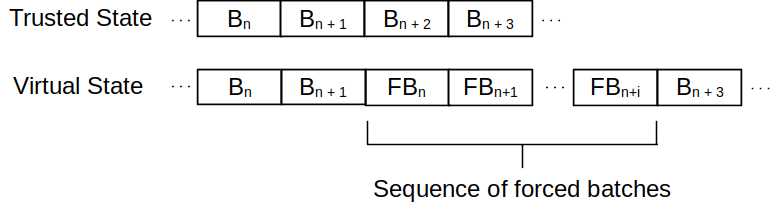
\includegraphics[scale=0.50]{\statemanagementdir/figures/forced-batches-l2-state-reorg.png}
	
	\captionof{figure}{Differences between trusted and virtual L2 State.}
\end{center}


 
\section{Resistance to Trusted Aggregator inactivity or malfunction}

As with the batches sequencing, the system described above will not have finality in case of absence or malfunction of the Trusted Aggregator since the L2 State transitions would never be consolidated in L1. For this reason, L1 PolygonZkEVM.sol contract has a function named \textbf{verifyBatches} that allows anyone to aggregate sequences of batches.

\begin{lstlisting} [language=Solidity]
	function verifyBatches(
		uint64 pendingStateNum,
		uint64 initNumBatch,
		uint64 finalNewBatch,
		bytes32 newLocalExitRoot,
		bytes32 newStateRoot,
		uint256[2] calldata proofA,
		uint256[2][2] calldata proofB,
		uint256[2] calldata proofC
	) public ifNotEmergencyState
\end{lstlisting}

As can be seen, \textbf{veifyBatches} function take same arguments as \textbf{trustedVerifyBatches}, nevertheless, \textbf{verifyBatches} has two more restrictions for a sequence to be aggregated, furthermore introduce a new L2 State stage named pending state. In addition to the conditions needed in \textbf{trustedVerifyBatches} the following conditions must also meet in \textbf{veifyBatches}:

\begin{itemize}
	\item The contract must to not be in emergency state.
	\item A \textbf{trustedAggregatorTimeout} storage variable delay must be passed from the timestamp of the last batch in the sequence (timestamp of when the batch was sequenced). \textbf{trustedAggregatorTimeout} variable is set by the contract's Admin. 
\end{itemize}

If all the conditions are met, the function will verify the Zero-Knowledge CI proof by calling \textbf{\_verifyAndRewardBatches} internal function and if the verification succeeds, unlike what the function \textbf{trustedVerifyBatches} would do, the sequence will not be aggregated instantly. The sequence verified will be added to \textbf{pendingStateTransitions} mapping awaiting to be aggregated during a time delay set by \textbf{pendingStateTimeout}.

\begin{lstlisting} [language=Solidity]
	// pendingStateNumber --> PendingState
	mapping(uint256 => PendingState) public pendingStateTransitions;
\end{lstlisting}



\begin{lstlisting} [language=Solidity]
	struct PendingState {
		uint64 timestamp;
		uint64 lastVerifiedBatch;
		bytes32 exitRoot;
		bytes32 stateRoot;
	}
\end{lstlisting}

Verified sequences of batches will be in an intermediary state called pending state, in which their state transition has not yet been consolidated, hence, the new L2 State root has not been added to \textbf{batchNumToStateRoot} mapping nor the bridge's new Global Exit Root has been updated. The \textbf{lastPendingState} storage variable will track the number of pending state transitions that are waiting to be consolidated and will be used as the key of the entry in the mapping. Since the Zero-Knowledge proof has been verified, the independent aggregator will still receive the aggregation reward.

Figure 11 shows the L2 Stages timeline from a batch perspective and the actions that triggers its inclusion to the next L2 State stage when a batch sequence is Aggregated through \textbf{veifyBatches} function. 
\begin{center}
	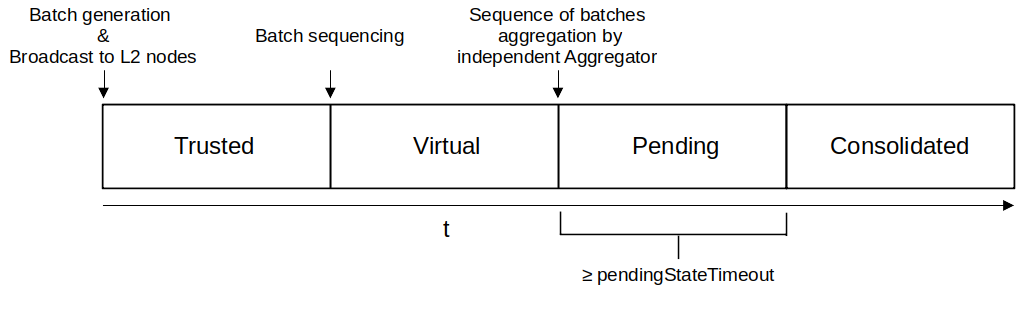
\includegraphics[scale=0.4]{\statemanagementdir/figures/pending-state.png}
	
	\captionof{figure}{L2 State stages timeline with pending state.}
\end{center}


The presence of sequences of batches in pending state do not affect to the correct working of the protocol since further sequences will be verified ahead pending ones. The \textbf{lastVerifiedBatch} storage variable will track the index of last batch verified and aggregated. Therefore, when a sequence of batches is pretended to be verified, the index of last verified batch will be queried through a function called \textbf{getLastVerifiedBatch}. This function will return the index of the last batch in the pending state if there are pending state transitions, or \textbf{lastVerifiedBatch} if there are not.

\begin{lstlisting}[language=Solidity]
	 function getLastVerifiedBatch() public view returns (uint64)
\end{lstlisting}

Each time the \textbf{sequenceBatches} function is called, an attempt to consolidate the pending state will be made  by calling \textbf{\_tryConsolidatePendingState} internal function. \textbf{\_tryConsolidatePendingState} will check if \textbf{pendingStateTimeout} has passed since pending state sequence of batches verification was made and will consolidate the pending state transitions if it. The Zero-Knowledge CI proof has already verified, therefore there is no need to verify its validity again.

Moreover, anyone can trigger the consolidation of a pending state by calling \textbf{consolidatePendingState} external function. If the caller account of \textbf{consolidatePendingState} is the trusted Aggregator account pending sequences of batches will be aggregate directly even if \textbf{pendingStateTimeout} has not passed since its verification. Else, if the caller account is not the trusted Aggregator account \textbf{consolidatePendingState} function will check if \textbf{pendingStateTimeout} has passed since pending state sequence of batches verification was made and will consolidate the pending state transitions if it.

\begin{lstlisting} [language=Solidity]
	function consolidatePendingState(uint64 pendingStateNum) external
\end{lstlisting}

With this mechanism is intended to give leeway to Polygon team in case of detection of soundness vulnerabilities exploitation in the Zero-Knowledge proof verification system and protect the assets from being bridged out the L2 by a malicious actors.




\section{Upgradability}

To allow for future updates to the protocol implementation (either in the case of adding new features, fixing bugs, or optimizations upgrades), the following contracts are deployed using a Transparent Upgradeable Proxy (TUP) pattern:

\begin{itemize}
	\item \textbf{PolygonZkEVM.sol.}
	\item \textbf{PolygonZkEVMGlobalExitRoot.sol.}
	\item \textbf{PolygonZkEVMBridge.sol.}
\end{itemize}

To inherit security and avoid prolonging and making the audit process more complex, the Polygon team has chosen to use the OpenZeppelin's openzeppelin-upgrades library in order to implement this functionality. OpenZeppelin has gained a reputation as a well-known brand in the industry because of its audits and open-source libraries of implementations of Ethereum standards, and its openzeppelin-upgrades library has been already audited and battle tested. Furthermore, openzeppelin-upgrades is not only a set of contracts but has also Hardhat and Truffle plugins to support the deployment, upgrades and administrator rights management of the proxies.

As can be seen in Figure 12, Open Zeppelin's TUP pattern, through the use of delegated calls and the fallback function, separates the protocol implementation of storage variables, thus providing the ability to update the implementation code without altering the storage state or changing the public address of the contract.

\begin{center}
	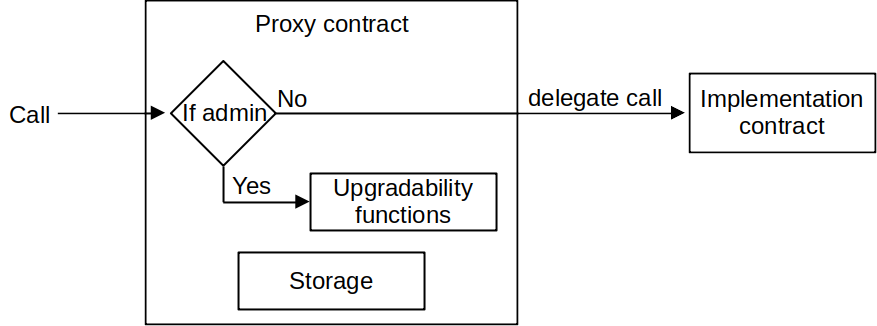
\includegraphics[scale=0.4]{\statemanagementdir/figures/OZ-transparent-proxy.png}
	
	\captionof{figure}{Open Zeppelin Transparent Upgradeable Proxy pattern schema.}
\end{center}

By following OpenZeppelin's recommendations, an instance of a contract called ProxyAdmin.sol, which is also included in the openzeppelin-upgrades library, is deployed and its address is set as the admin of the proxy contract. These operations can be done safely and easily using the Hardhat and Truffle plugins. Each ProxyAdmin.sol instance serves as the actual administrative interface for each proxy and the owner of each ProxyAdmin.sol instance will be the administrative account. ProxyAdmin.sol ownership will be transferred to the Admin role of the protocol (detailed in Section IX) during the deployment.

\section{Admin Role and Governance System}

The Admin is an Ethereum account to govern the entire protocol. Is the only account that can call the following functions set of the PolygonZkEVM.sol contract:

\begin{itemize}
	\item \textbf{setTrustedSequencer.}
	\item \textbf{setForceBatchAllowed.}	
	\item \textbf{setTrustedSequencerURL.}
	\item \textbf{setTrustedAggregator.}
	\item \textbf{setTrustedAggregatorTimeout.}
	\item \textbf{setPendingStateTimeout.}
	\item \textbf{setMultiplierBatchFee.}
	\item \textbf{setVeryBatchTimeTarget.}
	\item \textbf{setAdmin.}
	\item \textbf{deactivateEmergencyState.} 
\end{itemize}

Moreover, the Admin account is the owner of all ProxyAdmin.sol instances, that is, the unique account that can perform upgrade operations of protocol's contracts implementations.

Additionally, the Admin account holds ownership of all proxies, which means it is the unique account allowed of performing upgrades on the protocol's contracts implementations.

To increase the security and confidence of users when using the protocol, a timelock controller has been implemented. A timelock controller is a contract that allows to setup a delay to give a leeway to users to exit before a potentially dangerous maintenance operation is applied. A timelock controller allows to an admin to schedule and commit the maintenance operations transactions in L1, and when a given \textbf{minDelay} time expires, the timelock can be triggered to execute the maintenance operations transactions.

To inherit security and avoid prolonging and making the audit process more complex, the Polygon team has chosen to use the OpenZeppelin's battle tested TimelockController.sol contract, but with \textbf{getMinDelay} function overridden, this custom version of the OpenZeppelin's implementation is named PolygonZkEVMTimelock.sol. The new \textbf{getMinDelay}  will set the time \textbf{minDelay} to 0 in case of that emergency mode of the zkevm contract system is active (detailed in section X). The protocol's Admin role is set to an instance of PolygonZkEVMTimelock.sol contract address during the deployment. 

The Admin role requires significant responsibility and cannot be assigned solely to one account. For this reason, the Admin Ethereum account of a PolygonZkEVMTimelock.sol contract instance is assigned to a multi-sign contract that acts as a governance tool for the protocol, decentralizing the management power among multiple trusted entities.

Figure 13 shows the shape of the governance tree of Polygon zkEVM L1 contracts.

\begin{center}
	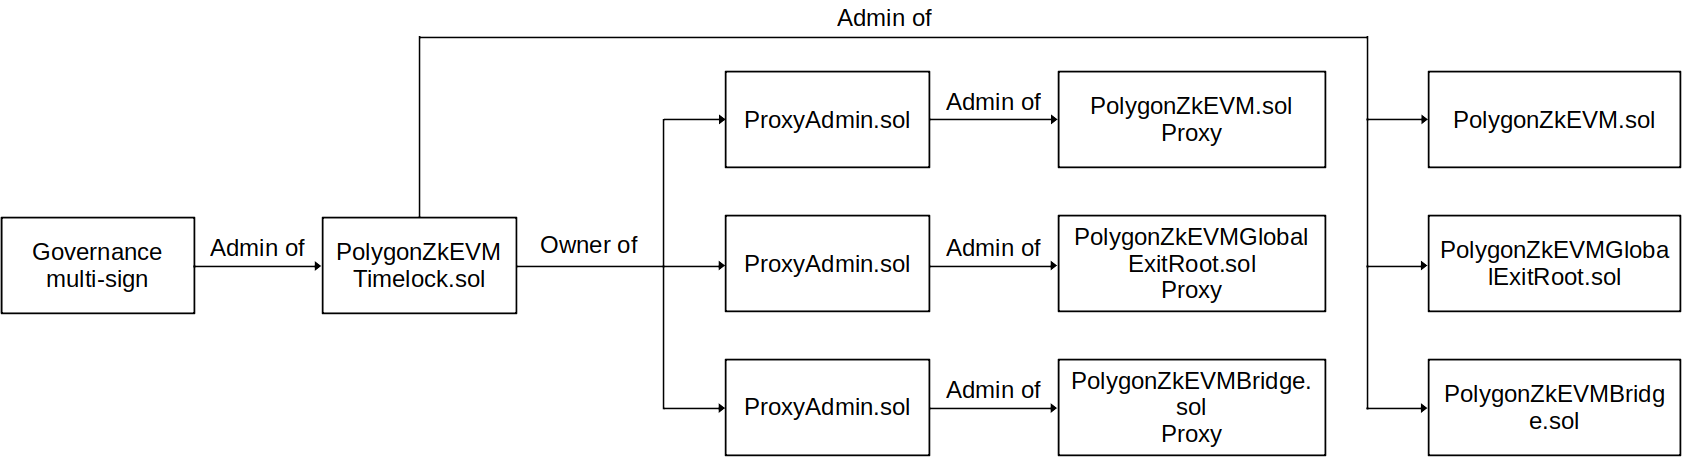
\includegraphics[scale=0.26]{\statemanagementdir/figures/Governance-chain.png}
	
	\captionof{figure}{Governance tree of Polygon zkEVM L1 contracts.}
\end{center}

In summary, protocol maintenance operations can only be performed by following these steps:

\begin{enumerate}
	\item Maintenance operations transactions are proposed and stored into governance multi-sign contract. Polygon team reaches a consensus whether applies or not these operation. Voting inherits security from L1.
	
	\item Once a decision has reached, if the results are favorable to perform maintenance operations, the governance multi-sing can be triggered to schedule thus transactions to be executed once a time delay has passed using PolygonZkEVMTimelock.sol contract instance.
	
	\item Once a time delay has passed PolygonZkEVMTimelock.sol contract instance can be triggered to execute scheduled transactions and fulfill maintenance operations.
\end{enumerate}



Note that due the governance chain among contracts any transaction on behalf of the Admin role can only be done through the above steps.
     
\section{Soundess attack resistance and emergency state}

The emergency state is a PolygonZkEVM.sol and PolygonZkEVMBridge.sol L1 contract state that when it is activated, batches sequencing and bridge operations will stop. The objective of this state is to give a leeway to the Polygon team to solve cases of soundness vulnerabilities exploitation or smart contract bugs exploitation and secure the L2 user's assets.

The following set of functions is locked while the contract is in emergency state:

\begin{itemize}
	\item \textbf{sequenceBatches}.
	\item \textbf{verifyBatches}.
	\item \textbf{consolidatePendingState} (Only if caller is  different from trusted Aggregator account).
	\item \textbf{forceBatch}.
	\item \textbf{sequenceForceBatches}.
	\item \textbf{proveNonDeterministicPendingState}.
\end{itemize}


Note that the Sequencer cannot sequence batches while the contract is in an emergency state. However, the trusted Aggregator will still be able to consolidate further state transitions or override a pending state transition that can be proved to be non-deterministic.

A non-deterministic state transition will occur when the same sequence of batches is successfully verified with two different resulting L2 State root values. This situation could arise from the exploitation of a soundness vulnerability in the verification system of the Zero-Knowledge CI proof.

Emergency state can only be triggered by two contract functions:

\textbf{activateEmergencyState}	will activate the emergency state directly if it is called by the contract owner. The contract owner is a different Ethereum account from the Admin account and is meant to eventually be abolished as it represents a bypass in the governance chain. However, it is only capable of triggering emergency state activation. Also can be called by everyone when a \textbf{HALT\_AGGREGATION\_TIMEOUT} constant delay (1 week) has passed since the batch corresponding to \textbf{sequencedBatchNum} argument has been sequenced but has not been verified yet. Note that this situation will mean that no one is aggregating sequences of batches, and the objective is to temporarily halt the protocol until aggregation activity can resume again.
\begin{lstlisting} [language=Solidity]
	function activateEmergencyState(uint64 sequencedBatchNum) external	
\end{lstlisting}
	
Additionally, anyone can trigger the emergency state if it is able to prove that some pending state is non-deterministic, using the \textbf{proveNonDeterministicPendingState} function.

\begin{lstlisting}
	function proveNonDeterministicPendingState(
		uint64 initPendingStateNum,
		uint64 finalPendingStateNum,
		uint64 initNumBatch,
		uint64 finalNewBatch,
		bytes32 newLocalExitRoot,
		bytes32 newStateRoot,
		uint256[2] calldata proofA,
		uint256[2][2] calldata proofB,
		uint256[2] calldata proofC
	) public ifNotEmergencyState
\end{lstlisting}



 If a soundness vulnerability exploitation is detected the Trusted Aggregator will be able to override a non-deterministic pending state. \textbf{overridePendingState} function is used to that proposit. Since the Trusted Aggregator is a trusted entity for the system, in the presence of a non-deterministic state transition, only the L2 state root provided by the Trusted Aggregator will be considered valid for consolidation.
  
 \begin{lstlisting} [language=Solidity]
 	function overridePendingState(
 		uint64 initPendingStateNum,
 		uint64 finalPendingStateNum,
 		uint64 initNumBatch,
 		uint64 finalNewBatch,
 		bytes32 newLocalExitRoot,
 		bytes32 newStateRoot,
 		uint256[2] calldata proofA,
 		uint256[2][2] calldata proofB,
 		uint256[2] calldata proofC
 	) public onlyTrustedAggregator
 \end{lstlisting}
 
  To successfully override pending state Trusted Aggregator must submit a proof that will be verified as in the \textbf{proveNonDeterministicPendingState} function, and if it succeeds, the pending state transition will be wiped and a new one will be consolidated directly.
 
 To sum up, emergency state can be triggered:
 \begin{itemize}
 	\item When the owner of the contract deems it appropriate.
 	\item When the aggregation activity is stopped for \textbf{HALT\_AGGREGATION\_TIMEOUT} time period (1 week))
 	\item When anyone is able to proof that a pending state is non-deterministic. 
 \end{itemize} 


\ifNOPOLYGON
\section{Questions}
\textbf{The individual validity of each transaction is not checked. What would happen in the event that transactions with an invalid format are sequenced?}

The aggregator should be able to prove that a transaction is invalid, meaning that even if the transaction is invalid, the Zero-Knowledge proof and the state transition in which that transaction is included remain valid. This allows for an invalid transaction to still be successfully sequenced and aggregated.

\textbf{If trustedAggregatorTimeout and veryBatchTimeTarget are valued nearby then all batches verified by independent aggregator will be above target (totalBatchesAboveTarget) and this would impact batch fees making them grow continuously. Isn't this situation a problem in the protocol?}

\textbf{trustedAggregatorTimeout} value is only meant to be high at initial stages and emergency time, during which 3rd party aggregation should not happen, thus preventing the issue. For time part from initialization and emergency, \textbf{trustedAggregatorTimeout} is meant to move towards 0 value. Moreover, Admin should always take care to set \textbf{trustedAggregatorTimeout} value lower than \textbf{veryBatchTimeTarget} during normal scenario to avoid this issue.

\textbf{As long are there is one Trusted Sequencer and one Trusted Aggregator the availability risks are relatively high. However the current code isn't optimized to support multiple Trusted Sequencers and multiple Trusted Aggregators. What solutions will be implemented to support multiple Trusted entities in the future?}

Since the \textbf{trustedSequencer}/\textbf{trustedAggregator} address can be changed, if we want to support multiple trusted actors or/and add a consensus layer to coordinate them this will be delegated in a future by another smart contract.

\section{TODO}
\begin{itemize}
\item Intro about L2 scalability solutions.
\end{itemize}
\fi